\documentclass[11pt,oneside]{article}
\usepackage[T1]{fontenc}
\usepackage[utf8]{inputenc}
%\DeclareUnicodeCharacter{00A0}{ }
\usepackage[adobe-utopia]{mathdesign}

\usepackage{amsmath}
\usepackage[francais]{babel}
\usepackage[dvips]{graphicx}
%\usepackage{here}
\usepackage{framed}
\usepackage[normalem]{ulem}
\usepackage{fancyhdr}
\usepackage{titlesec}
\usepackage{vmargin}

\usepackage{amsmath}
\usepackage{ifthen}
\usepackage{multirow}
\usepackage{multicol} % Portions de texte en colonnes

%\usepackage{xltxtra} % Logo XeLaTeX
%\usepackage{pst-solides3d}
\usepackage{color}
%\usepackage{colortbl}
\usepackage{titletoc} % Pour la mise en forme de la table des matières

%\usepackage[crop=off]{auto-pst-pdf}
%\usepackage{bclogo}


%\usepackage{longtable}
%\usepackage{flafter}%floatants après la référence
%\usepackage{pst-solides3d}
%\usepackage{pstricks}
%\usepackage{minitoc}
%\setcounter{minitocdepth}{4}
%\usepackage{draftcopy}% "Brouillon"
%\usepackage{floatflt}
%\usepackage{psfrag}
%\usepackage{listings} % Permet d'insérer du code de programmation
%\usepackage{lmodern}
%\usepackage[adobe-utopia,uppercase=upright,greeklowercase=upright]{mathdesign}
%\usepackage{minionpro}
%\usepackage{pifont}
%\usepackage{amssymb}
%\usepackage[francais]{varioref}

\setmarginsrb{1.5cm}{1cm}{1cm}{1.5cm}{1cm}{1cm}{1cm}{1cm}

\definecolor{gris25}{gray}{0.75}
\definecolor{bleu}{RGB}{18,33,98}
\definecolor{bleuf}{RGB}{42,94,171}
\definecolor{bleuc}{RGB}{231,239,247}
\definecolor{rougef}{RGB}{185,18,27}
\definecolor{rougec}{RGB}{255,230,231}
\definecolor{vertf}{RGB}{103,126,82}
\definecolor{vertc}{RGB}{220,255,191}
\definecolor{violetf}{RGB}{112,48,160}
\definecolor{violetc}{RGB}{230,224,236}
\definecolor{jaunec}{RGB}{220,255,191}
\usepackage[final]{pdfpages} 
\usepackage[%
    pdftitle={TD Conception},
    pdfauthor={Xavier Pessoles},
    colorlinks=true,
    linkcolor=blue,
    citecolor=magenta]{hyperref}



% \makeatletter \let\ps@plain\ps@empty \makeatother
%% DEBUT DU DOCUMENT
%% =================
\sloppy
\hyphenpenalty 10000

\newcommand{\Pointilles}[1][3]{%
\multido{}{#1}{\makebox[\linewidth]{\dotfill}\\[\parskip]
}}


\begin{document}


\newboolean{prof}
\setboolean{prof}{false}
%------------- En tetes et Pieds de Pages ------------
\pagestyle{fancy}
\renewcommand{\headrulewidth}{0pt}

\fancyhead{}
\fancyhead[L]{%
\begin{minipage}[c]{1.6cm}

\includegraphics[width=2cm]{png/logo_ptsi.png}%
\end{minipage}
\rule{2cm}{.5pt}
}

\fancyhead[C]{\rule{11cm}{.5pt}}

\fancyhead[R]{%
\begin{minipage}[c]{3cm}
\begin{flushright}
\footnotesize{\textit{\textsf{Sciences Industrielles\\ pour l'Ingénieur}}}%
\end{flushright}
\end{minipage}
}

\renewcommand{\footrulewidth}{0.2pt}

\fancyfoot[C]{\footnotesize{\bfseries \thepage}}
\fancyfoot[L]{\footnotesize{2012 -- 2013} \\ X. \textsc{Pessoles}}
\ifthenelse{\boolean{prof}}{%
\fancyfoot[R]{\footnotesize{TD -- CI 4 -- Conception des mécanismes -- P}}
}{%
\fancyfoot[R]{\footnotesize{TD -- CI 4 -- Conception des mécanismes}}
}


%\begin{center}
%\textit{Centre d'intérêt}
%\end{center}


\begin{center}
 \huge\textsc{CI 4 -- Conception des mécanismes}
\end{center}


\begin{center}
 \large\textsc{Unite de taraudage}
\end{center}
\vspace{.5cm}

\begin{flushright}
\textit{D'après ressources de Jean-Pierre Pupier.}
\end{flushright}
%
%\begin{minipage}[c]{.45\linewidth}
%\begin{center}
%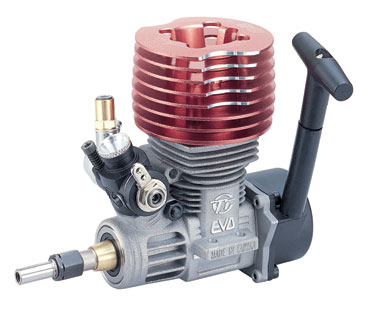
\includegraphics[height=3cm]{png/moteur}
%
%\textit{Moteur de modélisme}
%\end{center}
%\end{minipage}\hfill
%\begin{minipage}[c]{.45\linewidth}
%\begin{center}
%\includegraphics[height=4cm]{png/moteur_3D}
%
%\textit{Représentation d'un moteur de modélisme}
%\end{center}
%\end{minipage}

\begin{contexte}
\begin{itemize}
\item Objectif pédagogique : concevoir un système mécanique
\item Objectif technique : 
\begin{itemize}
\item Proposer une solution technologique permettant de concevoir une unité de taraudage
\end{itemize}
\end{itemize}
\end{contexte}

\section*{Présentation}

Cet appareil a pour fonction d'exécuter des trous taraudés. Le mouvement de rotation de l'arbre moteur 6 est transmis au taraud (implanté dans le cône Morse situé dans la partie droite de 4) sous la forme d'un mouvement de rotation (mouvement de coupe) et d'un mouvement de translation (mouvement d'avance).

La zone d'étude du dessin d'ensemble est représentée de façon schématique : elle sera à concevoir.

\section*{Questions}

\paragraph{}
\textit{Faire le schéma cinématique minimal de l'appareil complet en fonctionnement normal (le limiteur de couple 9,11,12,13 ne patine pas). Ne pas représenter le système de tension de la courroie.}

\paragraph{}
\textit{L'unité de taraudage doit pouvoir usiner des taraudages de pas quelconques P. Quel est le rapport entre le pas à exécuter P et le pas de la glissière hélicoïdale p de la zone d'étude encadrée ? Justifiez votre réponse.}

\paragraph{}
\textit{Que faudra-t-il faire comme manipulation sur le mécanisme existant pour adapter l'unité de taraudage à un pas P à exécuter différent ?}

\paragraph{}
\textit{On souhaite usiner un taraudage avec hélice à droite. Quel devra être le sens de l'hélice du système vis-écrou de la zone d'étude encadrée? Justifier votre réponse.}

\section*{Dessins}

On désire étudier la réalisation du sous-ensemble compris dans la zone d'étude encadrée.
 
\subsection*{Données}
\begin{itemize}
\item La longueur maximale du taraudage que ce dispositif va usiner est de 65 mm.
\item Le diamètre nominal du système vis-écrou que vous allez concevoir est de 16 mm.
\item Le système vis écrou devra être protégé des copeaux dus à l'opération de taraudage.
\item Le schéma indiqué étant cinématique minimal, il faut noter que les divers sous-ensembles qui le constituent pourront être réalisés technologiquement par plusieurs pièces.
\item Les manipulations destinées à préparer l'appareil pour effectuer des taraudages de pas P différents devront être simples et rapides.
\end{itemize}

\subsection*{Dessin}
\paragraph{}
\textit{Dessiner votre solution sur un calque au format A4.}
%Pour votre dessin penser au fait que le dessin d'ensemble est une réduction A2 $\rightarrow$ A3.}

\begin{center}
%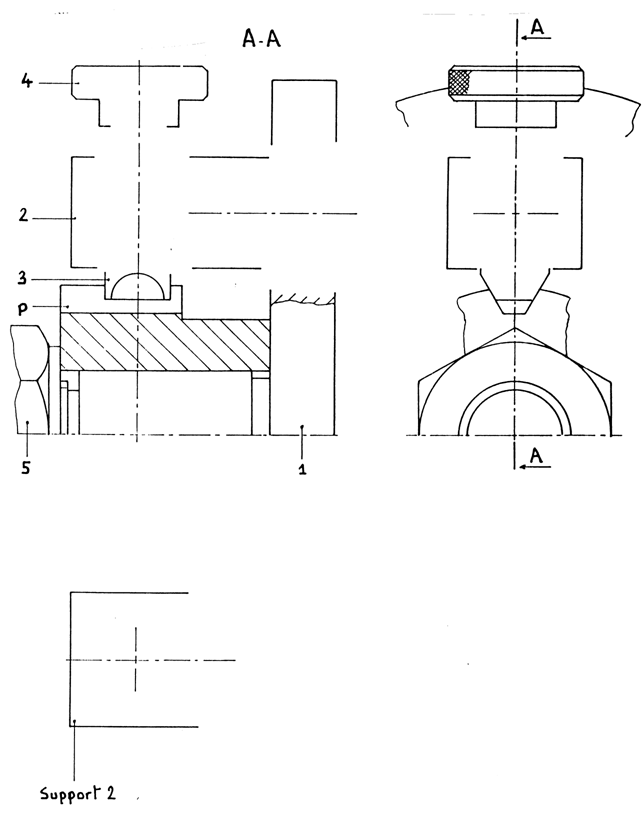
\includegraphics[width=.95\textwidth]{png/img5}
\end{center}

\end{document}